\documentclass{article}
\usepackage{wrapfig}
\usepackage{caption}
\usepackage{xcolor}
\usepackage{amsmath}
\usepackage{graphicx}
\usepackage{url}
\usepackage{subcaption}
\usepackage{placeins}
\captionsetup{justification=centering}\usepackage{graphicx} 
\usepackage{xcolor}
\usepackage[colorlinks=true, urlcolor={[HTML]{145680}}]{hyperref}
\usepackage{titlesec}
\usepackage[a4paper,left=1in,right=1.1in,top=1.1in,bottom=1in]{geometry}
\linespread{1.05}
\raggedbottom

\title{\Huge Three Utilities Problem \\[0.5em] \Large A Classic Puzzle Explored Through Graph Theory}

\author{Charlie Richley}
\date{}

\begin{document}

\maketitle
\large
\section{Problem statement}
\label{sec:problem_statement}
\setlength{\parindent}{0pt}
\setlength{\parskip}{1em}
\begin{minipage}[t]{0.52\textwidth}
\setlength{\parindent}{0pt}
\setlength{\parskip}{1em}
Imagine that \textit{you} are in charge of providing utilities to a city. 

You have three houses, and three utilities to provide them with (water, gas and electricity). You must connect each house to each utility by a wire.

The catch: can you do it without crossing over any of the wires?

Think about the problem, maybe try and sketch out some possibilities (though not for longer than a couple minutes!). Do you think it is possible? Why, or why not? This is what we will explore today. 
\end{minipage}
\hfill
\begin{minipage}[t]{0.45\textwidth}
\vspace{0pt}
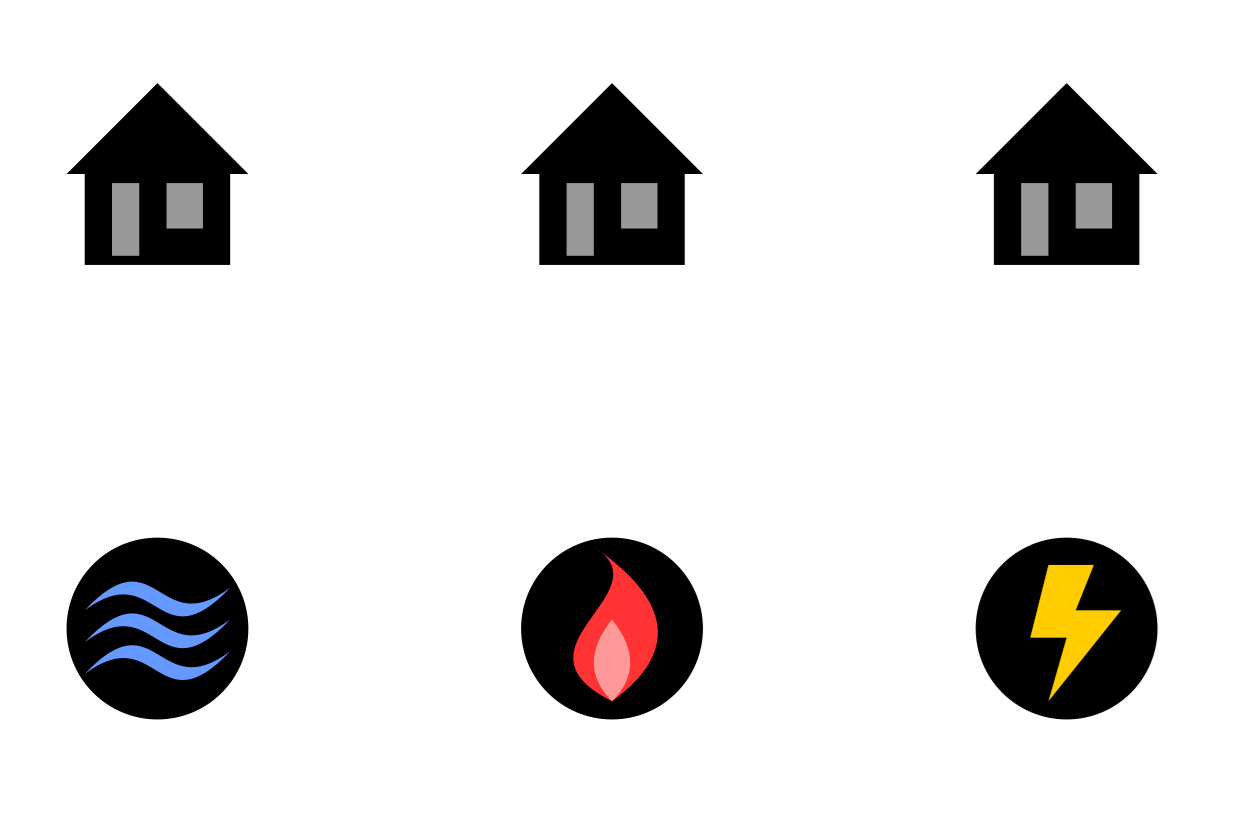
\includegraphics[width=\textwidth]{problem_statement.png}
\captionof{figure}{Can you find a way to connect each house to each utility, without any wires crossing?}
\end{minipage}

\section{An Introduction to Graph Theory}
\subsection{Motivations}
Whilst providing a solution to a classic problem, I aim to build a proof from first principles, assuming no results or theorems. We will solve this problem using graph theory, though there are other ways to get the same result.
\subsection{What is a graph?}
\noindent
\begin{minipage}[t]{0.58\textwidth}
\vspace{0pt}
I know what you are probably thinking... and no, it's not to do with plotting x-y graphs of equations!\\

Most simply, a graph is just dots connected by lines in a plane (though a mathematician may say a graph consists of vertices and edges). Edges in a graph split the plane into different regions (also called faces). \\

Graph Theory is a vast discipline, and many different types of graphs exist - we will look at planar, and connected planar graphs.

\end{minipage}\hfill
\begin{minipage}[t]{0.4\textwidth}
\vspace{-10pt}
\centering
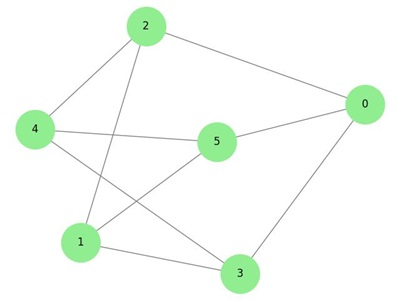
\includegraphics[width=\linewidth]{example_graph.jpg}
\captionof{figure}{An example of a graph with 6 vertices, 9 edges, and 8 regions}
\end{minipage}

\subsection{What might a graph look like that solves the Three Utilities Problem?}
\label{sec:might_look}
Well, we must have 6 vertices to represent the three houses and three utilities. There must be 9 edges in the graph, as each house has to connect to each utility.

\begin{figure}[h]
\centering
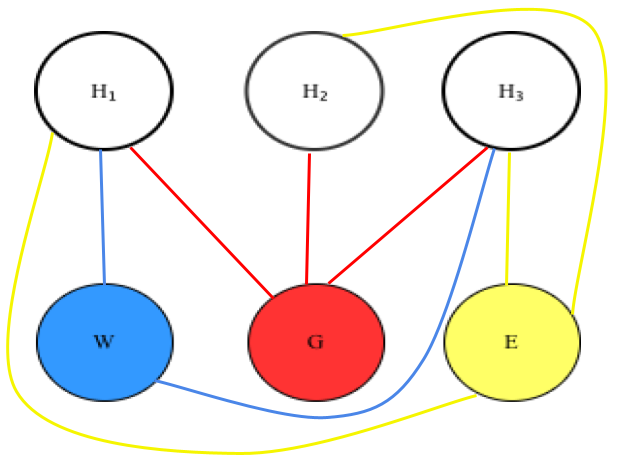
\includegraphics[width=0.45\textwidth]{graph_solution_idea.png}
\caption{How a graph to solve the Three Utilities problem could look like, with V = 6 and E = 9}
\label{fig:example_graph}
\end{figure}

Notice the fundamental flaw in the graph: the water is only connected to two of the three houses. It doesn't appear that there is a way to connect the water to $H_2$. This poses the question: is such a configuration even possible?
\section{Proving Euler's Formula for connected planar graphs}
\label{sec:euler_formula}
\subsection{What is a connected planar graph?}

A \textit{connected} graph is a graph where there exists a path between every possible pair of vertices.

\begin{wrapfigure}[8]{r}{0.4\textwidth}
\centering
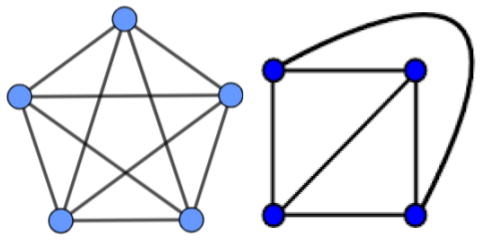
\includegraphics[width=\linewidth]{planar_vs_non_planar.png}
\caption{An example of non-planar (left) and planar graphs (right)}
\end{wrapfigure}

Whereas, a \textit{planar} graph is a graph which can be drawn in the 2D plane such that no edges intersect each other.

Determining whether a graph is planar can be quite tricky - though a graph may look non-planar if drawn in a weird way, there still could be a different way to draw the same graph without any edges crossing.

\subsection{What is Euler's formula?}

The first step in our solution is to prove Euler’s formula for connected planar graphs:
\begin{equation}
V - E + F = 2
\label{eq:euler}
\end{equation}
This equation describes a connected planar graph, with V vertices, E edges, and F faces (meaning how many different regions the plane is split into when the graph is drawn). 

It is quite a remarkable formula. The number of faces and vertices added together, subtract the number of edges is a constant, or invariant. Even if the graph looks weird, or is extremely large, the formula still holds.

Let’s try and prove it by mathematical induction: for us, this means showing that the formula works in a base case, and then showing that all other possible graphs can be reduced down to the base case. 

\subsection{The base case}
Consider the base case - a non-empty graph of minimum size, so 0 edges. The graph will contain only one vertex. Clearly, we can see that E = 0, V = 1, and F = 1 (because the only face in the graph is just the plane).

$V - E + F = 1 - 0 + 1 = 2$, so the formula holds in the base case.

\subsection{Reducing all possible graphs to the base case}
Let us assume that a connected planar graph G has V vertices, E edges and F faces. We will show that this graph can simply be reduced to the base case, which would mean our proof works for all graphs of this type (as we have already proven the base case).

\textbf{Definition:} A \textit{cycle} is a loop in the graph, starting and ending at the same vertex, without visiting any vertex more than once.

\subsection{Case 1: The edge is not part of a cycle}
We first consider an edge that connects two vertices, but is not part of a cycle in the graph. Let us remove this edge, and then combine those two vertices into just one vertex.

On the graph below, we remove the edge connecting vertices 3 and 5.

\begin{figure}[h]
\centering
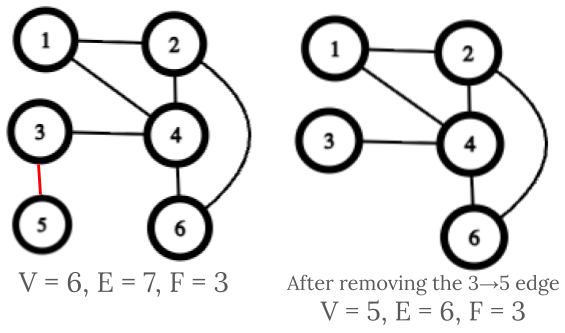
\includegraphics[width=0.6\textwidth]{case_1.png}
\caption{What happens when we remove an edge that is \textit{not} part of a cycle? (edge {\textcolor{red}{$3 \to 5$}})}
\end{figure}

Removing edge $3 \to 5$, and combining vertices 3 and 5 into vertex 3 leads to the graph on the right hand side. We can observe that this has not affected the number of regions in the graph, but simply has resulted in the loss of one edge ($3 \to 5$), and one vertex (number 5).

More generally, removing such an edge will reduce both the number of edges and vertices in the graph by one. Given that this edge was not part of a cycle, removing it will not change the number of regions (faces) in the graph. 

So, now we have E - 1 edges, V - 1 vertices, and F faces. 

Using our formula \eqref{eq:euler}:

$V - 1 - (E - 1) + F$ \; = \; $V - 1 - E + 1 + F$ 

Simplifying leads to $V - E + F$, so we can say that removing this edge did not change the value of $V - E + F$. It stayed constant, despite us removing an edge.

\subsection{Case 2: The edge is part of a cycle}
We now consider what happens when we remove an edge that is part of a cycle from the graph.
\\
\\
\\
\\

\begin{figure}[h]
\centering
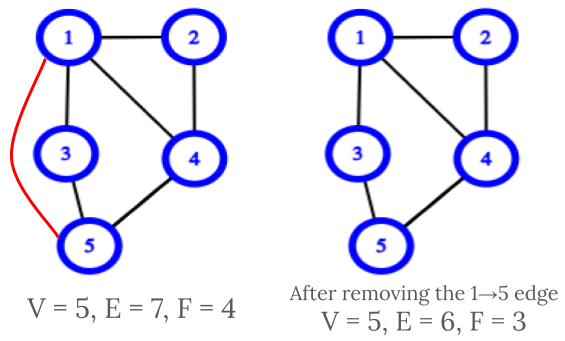
\includegraphics[width=0.6\textwidth]{case_2.png}
\caption{What happens when we remove an edge that \textit{is} part of a cycle? (edge {\textcolor{red}{$1 \to 5$}})}
\end{figure}
In this graph, we removed the edge connecting vertices 1 and 5. This edge was part of a cycle of $1 \to 3 \to 5$ (then back to 1). We can notice that removing this edge meant we lost a region, so F decreased by one, and of course removing an edge meant E decreased by one too. 

For the first graph, calculating $V - E + F$ gives $5-7+4 = 2$. \newline
After removing the edge, we now get $V - E + F = 5 - 6 + 3$, which is also equal to 2. 

What we notice here is that $V - E + F$ stays constant even when removing this edge.

Generalising our observations, removing such an edge will reduce the number of regions (faces) by one, because that edge used to separate two regions, but they are now merged together. Of course, it will also reduce the number of edges by one.

We now have V vertices, E - 1 edges, and F - 1 faces. 

Using our formula again: 

$V - (E - 1) + F - 1$\; = \;$V - E + 1 + F - 1$,

This simplifies to $V - E + F$ again, meaning removing an edge that was part of a cycle also did not change the value of $V -  E + F$.

\subsection{Looking at the bigger picture}
Think about what we have shown so far… Intuitively, an edge is either part of a cycle, or it isn’t. Full stop.

In each of the cases, we have shown that removing that edge does not affect the value V - E + F.

So, for any such graph that you could think of: simply keep removing edges (and combining vertices, if Case 1 applies), removing edges, removing edges (you get the point), and we know it won’t change V - E + F. After a lot of removing edges, you will finally reach the base case: a graph with one vertex, and no edges, which we have shown satisfies $V - E + F = 2$. 

Hence, we can conclude that our formula holds for ALL connected planar graphs.

Well, you are probably thinking: that’s a nice formula, but how could it possibly relate to our Three Utilities Problem?

We must now build off this formula to derive an inequality - which we can then apply to our graph involving the three houses and three utilities.

\section{Producing a solution to the Three Utilities Problem}
\subsection{Deriving the inequality \texorpdfstring{$E \leq 2V - 4$}{E =< 2V - 4}}
\label{subsec:inequal}
Our result from above~(\ref{eq:euler}) will come in handy here. In order to obtain our inequality, we must make a few assumptions: 
\vspace{-6pt}
\begin{itemize}
  \item[-] Our assumption is that there are no cycles of length 3 (triangles) in the graph. For the Three Utilities problem, this is true as there can only be a cycle with even length. This is because each edge must connect between a house and a utility, and you alternate sides every time you cross an edge (e.g. house, to utility, then back to house). If there is an odd number of edges in the cycle, you will be on the opposite side than you started on.
  \item[-]  We also say V $\geq 3$ (in our graph V = 6, so this is fine).
  \item[-] This applies only to simple planar graphs, meaning no edges overlap, no edges connect back to themselves in a loop, and there can only be a maximum of one edge between two given vertices.
\end{itemize}
\vspace{-6pt}

\textbf{Definition:} The degree of a region is the number of edges around it.
\begin{figure}[h]
\centering
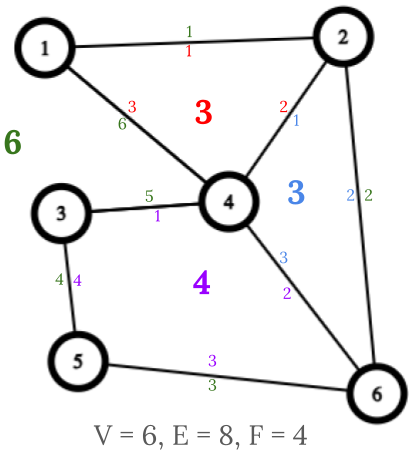
\includegraphics[width=0.348\textwidth]{sum_degrees.png}
\caption{Degree of each region in the centre of the region (bold). The smaller numbers are counting clockwise the number of edges that surround a particular region.}
\end{figure}

We can see that the sum of the degrees of each region in a graph is equal to twice the number of edges. Why? Well, each edge touches 2 regions (one on each side). So, when counting the degree of each region, you will count each edge twice overall. 

Figure 7 illustrates an example of this. It shows a graph with four regions, with the sum of the degrees of each region being $3 + 3 + 4 + 6 = 16$, and $16 / 2 = 8$, which we can notice is indeed the number of edges in this graph.

Therefore, we say that $\sum \mathrm{degrees} = 2E$.

Think about what defines a region: you would need not one, or two edges to enclose a region. You need three or above, but in the problem statement, we said there are no cycles of length 3, so the degree of each region must be $\geq 4$. 

This is a very important observation - this allows us to actually set up an inequality, which will help us to solve the problem.

The sum of the degrees of each region is 2E - this is an exact total, as we showed above.\newline
\textit{Exact total:} $2E$ 

Each possible region has a \textit{minimum} degree of 4, so multiplied by the number of regions F creates a lower bound for the sum of the degrees of each region.\newline
\textit{Lower bound:} $4F$ 

Comparing our lower bound and exact total gives $2E \geq 4F \implies \frac{1}{2}E \geq F$.

We know from earlier from Euler's formula~(\ref{eq:euler}) that $V - E + F = 2$.

Rearranging gives $F = E - V + 2$

Plugging the equation for F into our inequality gives $\frac{1}{2}E \geq E - V + 2$

Bringing the E to the right hand side gives $\frac{1}{2} E - V + 2 \leq 0$

Hence, $\frac{1}{2}E \leq V - 2$ , then multiplying through by 2 gives $E \leq 2V - 4$.

We have derived the most important inequality, which will (finally!) allow us to solve our problem.

Our inequality states that for all simple planar graphs (with no triangles and $V \geq 3$)
\begin{equation}
E \leq 2V - 4
\label{eq:inequality}
\end{equation}

\subsection{Is it actually possible to connect the houses to the utilities?}
As explained in \ref{sec:might_look}, we know our graph must have V = 6 and E = 9. 
\newline
Let’s plug this into our inequality, $E \leq 2V - 4$~(\ref{eq:inequality}).

$9 \leq 2(6) - 4$

$9 \leq 12 - 4$ $\implies$ $9 \leq 8$

Is 8 bigger than or equal to 9?

Clearly not! We have reached a contradiction - as our inequality holds for all planar graphs, and our graph doesn't satisfy it, it therefore cannot be planar.

Therefore, we can conclude that it is \textbf{impossible} to draw this graph without crossing over one of the edges, so it turns out that the problem has no solution after all!

\section{Reflection}
\subsection{Looking Beyond The Plane}
So far, we've been trying to solve our problem on a plane - equivalent to using pen and paper to join up our houses and utilities.

What if we look at the problem on another surface, say a coffee mug?

\captionsetup[subfigure]{labelformat=empty}
\begin{figure}[h]
\centering
\begin{subfigure}{0.45\textwidth}
\centering
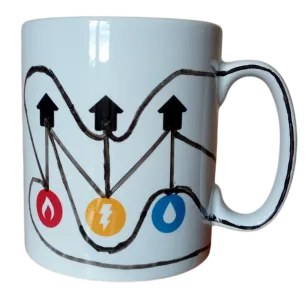
\includegraphics[width=\linewidth]{three_utilities_mug.png}
\caption{Solving the Three Utilities Problem on a different surface: a coffee mug}
\end{subfigure}
\hfill
\begin{subfigure}{0.45\textwidth}
\centering
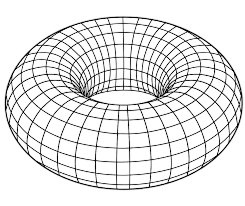
\includegraphics[width=\linewidth]{torus.png}
\caption{A torus - topologically equivalent to a coffee mug, and often called a doughnut}
\end{subfigure}
\end{figure}

In topology, an advanced and dangerously pure branch of Mathematics, there is a type of shape called a torus, a curved shape with a hole in the middle.

Topology studies the properties of shapes that remain unchanged despite being stretched, twisted or bent - it is unconcerned with angles or distance, unlike traditional geometry. 

Seeing as both a coffee mug and a torus both have one hole, we say they are topologically equivalent to one another.

So, on this new surface, it is now possible to join up the utilities and houses, as the hole (or coffee mug handle!) allows us to avoid  path crossings we couldn't before. With a different surface, we can now provide a solution to the problem.

\subsection{Reflecting on Graph Theory}
Clearly, graph theory is not a subject involving computing lots of challenging sums - the hardest calculation in this essay is solving a linear inequality!

Nonetheless, the great difficulties come with the challenging conceptual ideas, and moving from looking at a specific graph, to trying to generalise patterns that can sometimes feel quite abstract. 

Hopefully, you have found that visualising a problem is, more often than not, the key to solving it.

\section*{References}

\begin{itemize}
  \item     \url{https://sites.math.washington.edu/~julia/teaching/445_Spring2013/Paper_Euler.pdf} - Proof of the formula $V - E + F = 2$ (section~\ref{sec:euler_formula})
  \item \url{https://courses.grainger.illinois.edu/cs173/fa2009/lectures/lect_40.pdf} — Proof of the inequality $ E \leq 2V - 4$ (subsection~\ref{subsec:inequal})
  \item 
  \url{https://www.futilitycloset.com/2025/08/28/the-three-utilities-problem/} — Used in Figure 1
  \item \url{https://www.tutorialspoint.com/graph_theory/graph_theory_types_of_graphs.htm} — Used in Figure 2
  \item 
  \url{https://medium.com/math-simplified/graph-theory-101-why-all-non-planar-graphs-contain-k%E2%82%81-or-k%E2%82%83-%E2%82%83-c3ad48d6798e} — Used in Figure 4
  \item \url{https://www.boost.org/doc/libs/latest/libs/graph/doc/planar_graphs.html} — Used in Figure 4
  \item 
  \url{https://games4life.co.uk/tag/three-utilities-problem/} — Used in the last figure in Section 5
  \item \url{https://math.uchicago.edu/~may/REU2024/REUPapers/Courbe.pdf} 
  - Used in the last figure in Section 5
  \item \url{https://csacademy.com/app/graph_editor/} — Used to create my own figures for Figure 3, 5, 6 and 7

\end{itemize}

\end{document}